\chapter{Design of the Engine}

\section*{Specifications}

Following is the specification for the current storage of image and kernel data:-

\begin{itemize}

\item 8 bits per pixel of image data and also kernel data.
\item Image would be of size 1024 x 1024 pixels (Basically 1022x1022 with zero padding).
\item Kernel would be of size 3 x 3.

\end{itemize}

Following is the specification for the current convolution core:- 

\begin{itemize}

\item An AXI Slave interface as the input interface for the addresses for the fetcher.
\item The number of coprocessors are kept variable to compare performance and hardware resource consumption.
\item A FIFO like interface for the fetcher to interface with the convolution core.
\item An AXI Master port for the fetcher for performing write backs to the memory.

\end{itemize}

\section{Storage design for image data}

The data is stored row wise as shown in the figure below. This strategy was opted to make the fetch and write back protocol really
straight-forward. The core gets the address of the first element of the first row of the image matrix, and of the kernel matrix and also the
physical address of the write back location in the DRAM.

\section{Fetch policy for the engine}

The fetch policy for the core is includes fetching the kernel data first and sending it out to all the coprocessors inside the core. After
this the fetching of image data begins and here we play a little smart and fetch 4 bytes of data in every memory read call and split the
data within the core to segregate the individual pixel data. 

\section{Number of coprocessors}

Since the image is chosen to be of size 1024x1024 it seems really convenient to have a number of coprocessors which is a factor of 1024. To
keep it symmetric we have kept the number of coprocessors to be 1, 2, 4, 8, 16 and 32 so that a single model of coprocessor can be
replicated in an convenient manner. Each coprocessor is fed with x rows of image data and the coprocessors are started in parallel, here x is
dependent on the number of operational coprocessors in the design.

\section{Flow design}

Figure~\ref{convolution core} represents the internal flow of the generic convolution engine which employs a variable number of cores since
we will utilize this to employ this design to test the performance and hardware consumption on a range of number of coprocessors. As can be
seen the core has a fetch unit which is responsible for fetching the incoming data from the input pipe to the core and distributing the work
between all the operational cores one by one and then collecting back the results from each of their output pipes and writing it back to the output pipe
of the core. Each coprocessor is designed to convolve the incoming image data with an initially stored kernel and write back the result to
its respective output pipe. The coprocessor model is discussed later on and we also dive down into the internal design of the coprocessor
when we discuss about improving its design efficiency and throughput.

\begin{figure}[H]
\centering
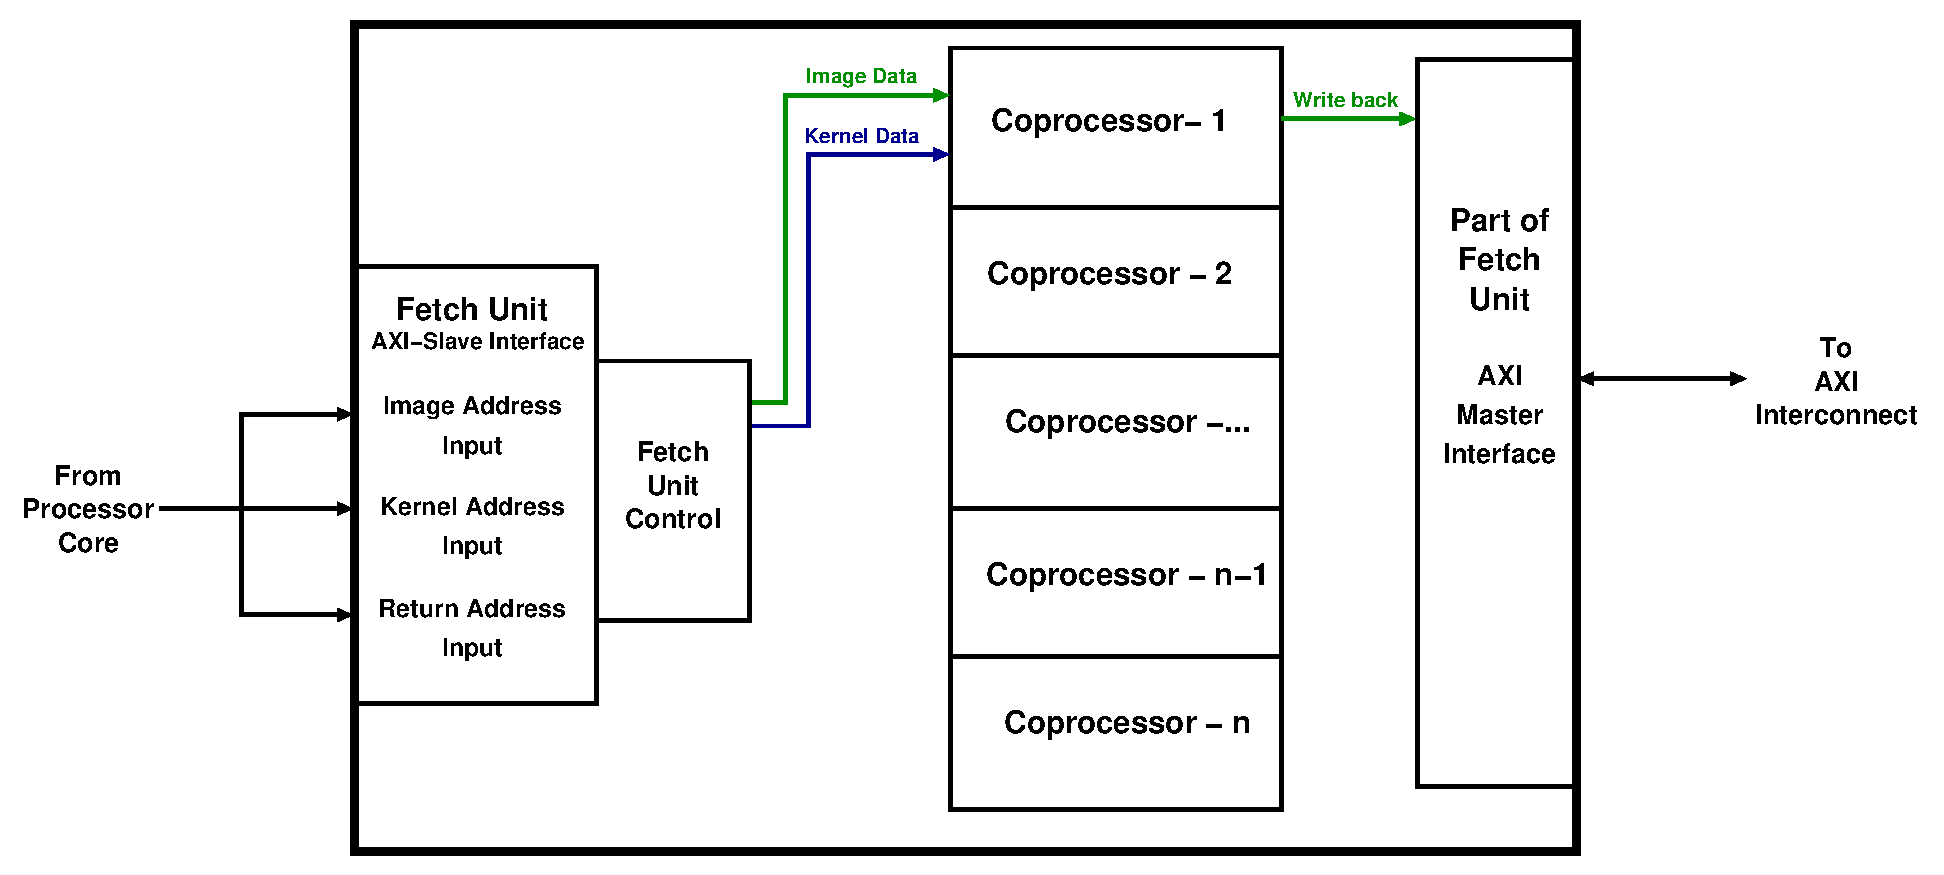
\includegraphics[scale=0.5]{eps_pdf_sources/convolution_engine/core}
\caption{Core Design}
\label{convolution core}
\end{figure}

\onehalfspacing
Figure~\ref{full system integrated with convolution engine} shows a sample system which could be built to integrate the convolution engine
with the AJIT FPGA system. The convolution engine can be controlled by AJIT and can also be directly tinkered with from the host machine
through the PCIe-AXI block. The engine can be assigned a task to perform a convolution from a software application by first storing the
relevant data in DRAM by \verb|write_to_axi_dram| call from the driver API and then the results can be read back using the
\verb|read_from_axi_dram| call.

\begin{figure}[H]
\centering
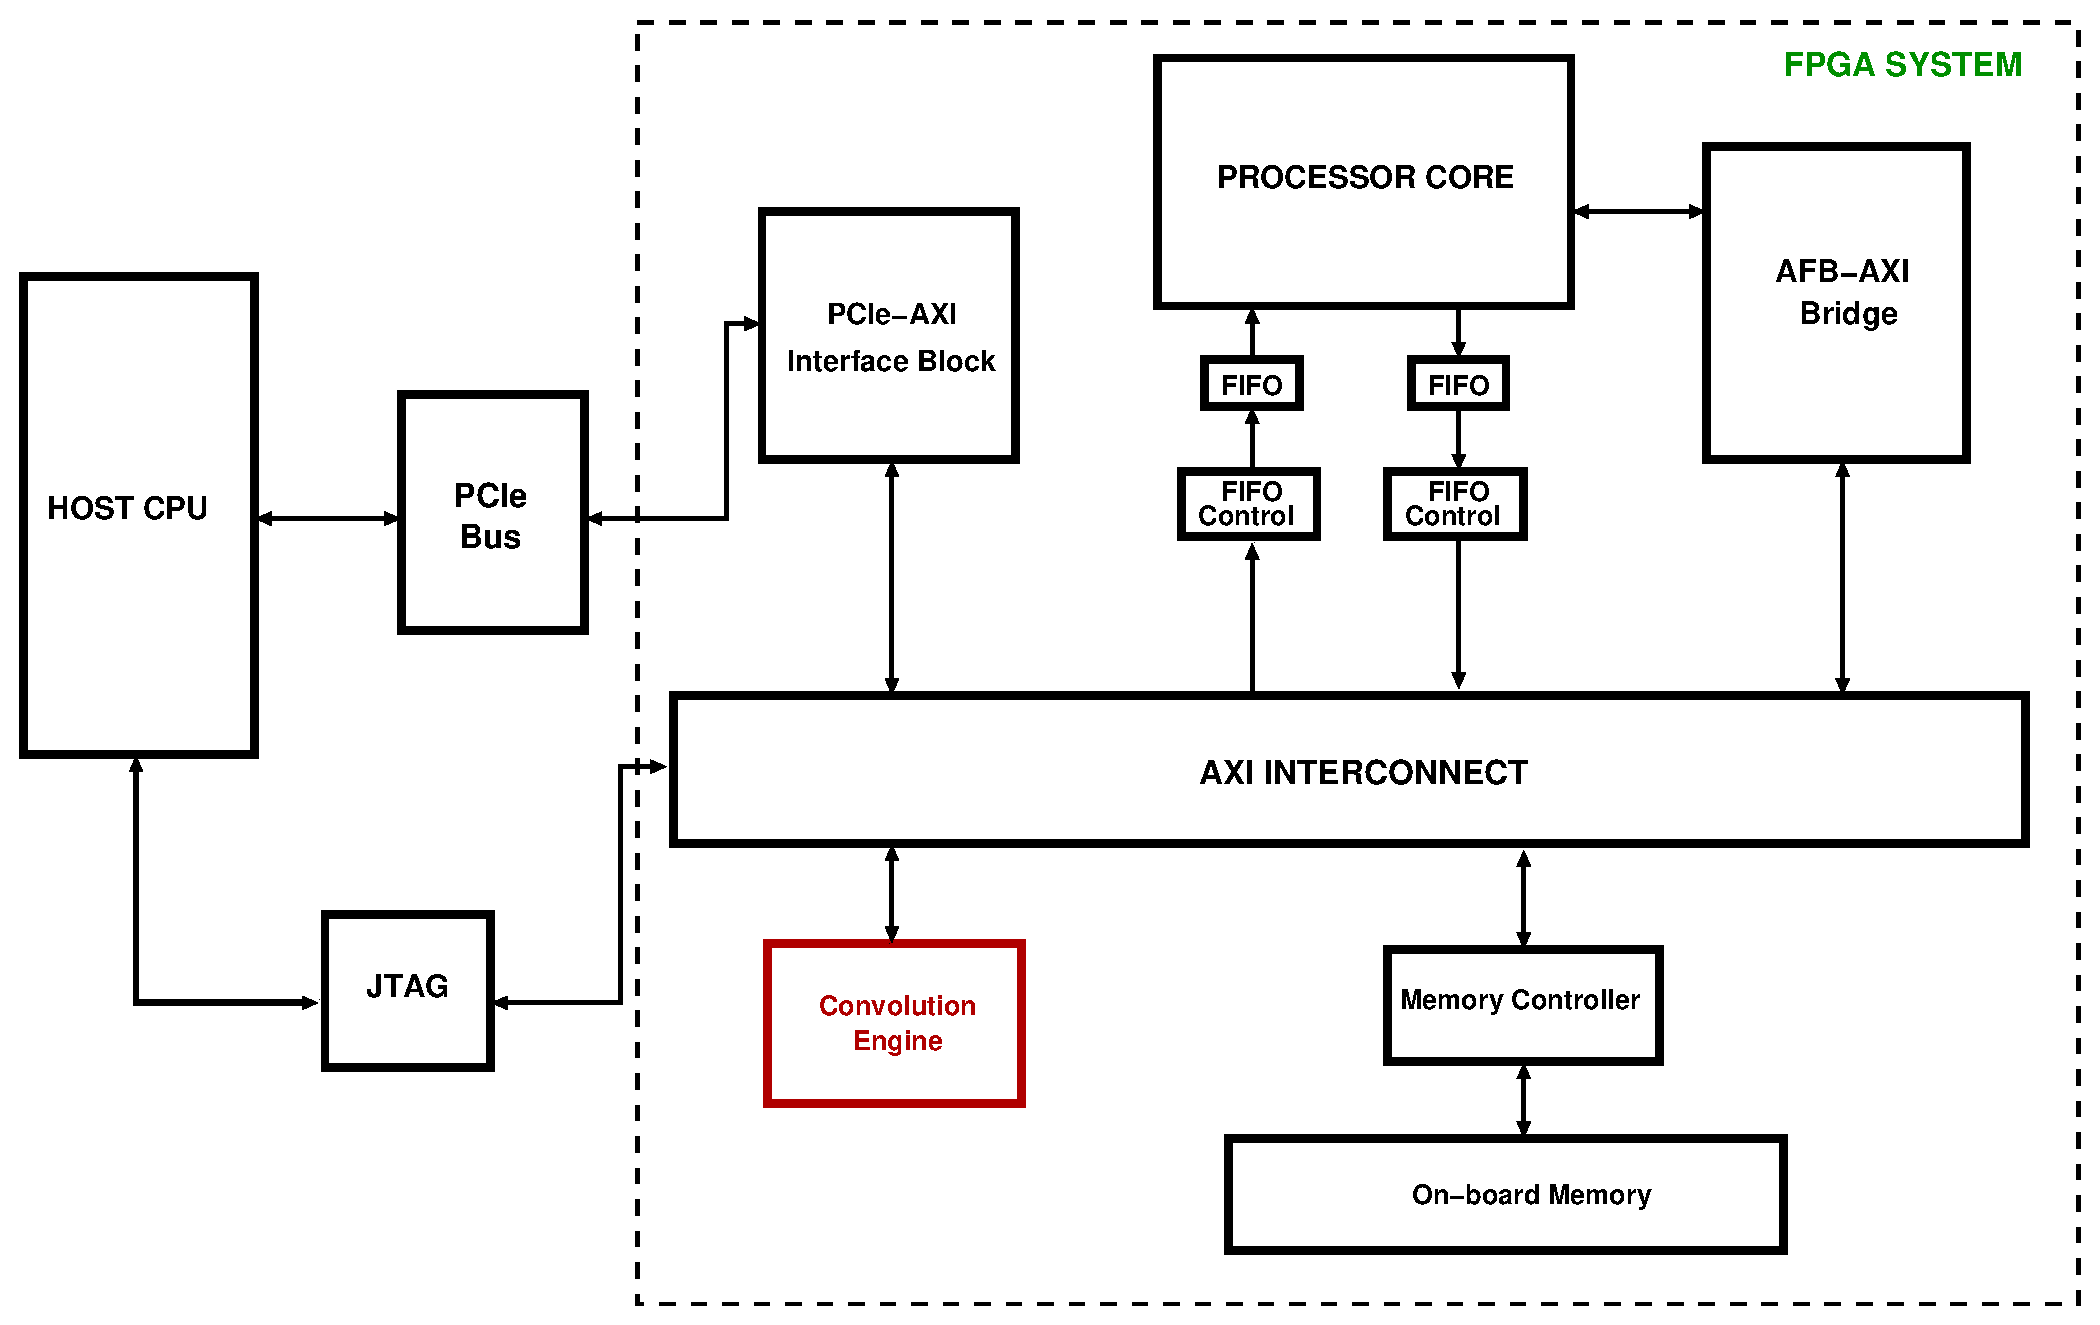
\includegraphics[width=\textwidth]{eps_pdf_sources/convolution_engine/Full_system_integrated_with_core}
\caption{Complete FPGA system with data flow}
\label{full system integrated with convolution engine}
\end{figure}

\doublespacing
